%
% Copyright 2014, General Dynamics C4 Systems
%
% This software may be distributed and modified according to the terms of
% the GNU General Public License version 2. Note that NO WARRANTY is provided.
% See "LICENSE_GPLv2.txt" for details.
%
% @TAG(GD_GPL)
%

\chapter{\label{ch:cspace}Capability Spaces}

Recall from \autoref{sec:cap-access-control} that seL4 implements a
capability-based access control model.  Each userspace thread has an
associated \emph{capability space} (CSpace) that contains the
capabilities that the thread possesses, thereby governing which
resources the thread can access.

Recall that capabilities reside within kernel-managed objects known as
\obj{CNode}s. A \obj{CNode} is a table of slots, each of which may
contain a capability. This may include capabilities to further
\obj{CNode}s, forming a directed graph. Conceptually a thread's CSpace
is the portion of the directed graph that is reachable starting with
the \obj{CNode} capability that is its CSpace root.

A CSpace address refers to an individual slot (in
some \obj{CNode} in the CSpace), which may or may not contain a
capability. Threads refer to capabilities in their CSpaces (e.g. when
making system calls) using the address of the slot that holds the
capability in question.  An address in a CSpace is the concatenation
of the indices of the \obj{CNode} capabilities forming the path to the
destination slot; we discuss this further in
\autoref{s:cspace-addressing}.

% FIXME The references to mint in the following paragraph and previously in
% this section need to be cleaned up. They were clearly written at a time when
% it was not possible to change a capability's rights during a CNode_Copy.
Recall that capabilities can be copied and moved within CSpaces, and
also sent in messages (message sending will be described in detail in
\autoref{sec:cap-transfer}).  Furthermore, new capabilities can be
\emph{minted} from old ones with a subset of their rights.  Recall,
from \autoref{s:memRevoke}, that seL4 maintains a \emph{capability
  derivation tree} (CDT) in which it tracks the relationship between
these copied capabilities and the originals.  The revoke method
removes all capabilities (in all CSpaces) that were derived from a
selected capability. This mechanism can be used by servers to restore
sole authority to an object they have made available to clients, or by
managers of untyped memory to destroy the objects in that memory so it
can be retyped.

seL4 requires the programmer to manage all in-kernel data structures,
including CSpaces, from userspace. This means that the userspace
programmer is responsible for constructing CSpaces as well as
addressing capabilities within them.  This chapter first discusses
capability and CSpace management, before discussing how capabilities
are addressed within CSpaces, i.e. how applications can refer to
individual capabilities within their CSpaces when invoking methods.

\section{Capability and CSpace Management}

\subsection{CSpace Creation}

CSpaces are created by creating and manipulating \obj{CNode} objects.
When creating a \obj{CNode} the user must specify the number of slots
that it will have, and this determines the amount of memory that it
will use. Each slot requires 16 bytes of physical memory and has the
capacity to hold exactly one capability. Like any other object, a
\obj{CNode} must be created by calling
\apifunc{seL4\_Untyped\_Retype}{untyped_retype} on an appropriate
amount of untyped memory (see \autoref{sec:object_sizes}).  The caller
must therefore have a capability to enough untyped memory as well as
enough free capability slots available in existing \obj{CNode}s for
the \apifunc{seL4\_Untyped\_Retype}{untyped_retype} invocation to
succeed.

\subsection{CNode Methods}
\label{sec:cnode-ops}

Capabilities are managed largely through invoking \obj{CNode} methods.

\obj{CNodes} support the following methods:
\begin{description}
\item[\apifunc{seL4\_CNode\_Mint}{cnode_mint}] creates a new
  capability in a specified \obj{CNode} slot from an existing
  capability.  The newly created capability may have fewer rights than
  the original and a different guard (see
  \autoref{sec:cap_address_lookup}). \apifunc{seL4\_CNode\_Mint}{cnode_mint}
  can also create a badged capability (see \autoref{sec:ep-badges})
  from an unbadged one.
\item[\apifunc{seL4\_CNode\_Copy}{cnode_copy}] is similar to
  \apifunc{seL4\_CNode\_Mint}{cnode_mint}, but the newly created
  capability has the same badge and guard as the original.
\item[\apifunc{seL4\_CNode\_Move}{cnode_move}] moves a capability
  between two specified capability slots. You cannot move a capability
  to the slot in which it is currently.
\item[\apifunc{seL4\_CNode\_Mutate}{cnode_mutate}] can move a
  capability similarly to \apifunc{seL4\_CNode\_Move}{cnode_move} and
  also reduce its rights similarly to
  \apifunc{seL4\_CNode\_Mint}{cnode_mint}, although without an
  original copy remaining.
\item[\apifunc{seL4\_CNode\_Rotate}{cnode_rotate}] moves two
  capabilities between three specified capability slots. It is
  essentially two \apifunc{seL4\_CNode\_Move}{cnode_move} invocations:
  one from the second specified slot to the first, and one from the
  third to the second. The first and third specified slots may be the
  same, in which case the capability in it is swapped with the
  capability in the second slot. The method is atomic; either both or
  neither capabilities are moved.
\item[\apifunc{seL4\_CNode\_Delete}{cnode_delete}] removes a
  capability from the specified slot.
\item[\apifunc{seL4\_CNode\_Revoke}{cnode_revoke}] is equivalent to
  calling \apifunc{seL4\_CNode\_Delete}{cnode_delete} on each derived
  child of the specified capability. It has no effect on the
  capability itself, except in very specific circumstances outlined
  in Section~\ref{s:cspace-revoke}.
\item[\apifunc{seL4\_CNode\_CancelBadgedSends}{cnode_cancelbadgedsends}] cancels
  any outstanding sends that use the same badge and object as the
  specified capability.
\end{description}

\subsection{Capabilities to Newly-Retyped Objects}
\label{sec:caps_to_new_objects}

When retyping untyped memory into objects with
\apifunc{seL4\_Untyped\_Retype}{untyped_retype}, capabilities to the
newly-retyped objects are placed in consecutive slots in a
\obj{CNode} specified by its \texttt{root}, \texttt{node\_index}, and
\texttt{node\_depth} arguments. The \texttt{node\_offset} argument specifies the
index into the \obj{CNode} at which the first capability will be placed.
The \texttt{num\_objects} argument specifies the number of capabilities (and, hence, objects)
to create. All slots must be empty or an error will result. All resulting
capabilities will be placed in the same \obj{CNode}.

\subsection{Capability Rights}
\label{sec:cap_rights}

As mentioned previously, some capability types have \emph{access
  rights} associated with them. Currently, access rights are
associated with capabilities for \obj{Endpoint}s (see
\autoref{ch:ipc}), \obj{Notification}s (see
\autoref{ch:notifications}) and \obj{Page}s (see \autoref{ch:vspace}).  The
access rights associated with a capability determine the methods that
can be invoked.  seL4 supports three orthogonal access rights, which
are Read, Write and Grant.  The meaning of each right is interpreted
relative to the various object types, as detailed
in~\autoref{tab:rights}.

When an object is first created, the initial capability that refers to
it carries the maximum set of access rights. Other, less-powerful
capabilities may be manufactured from this original capability, using
methods such as \apifunc{seL4\_CNode\_Mint}{cnode_mint} and
\apifunc{seL4\_CNode\_Mutate}{cnode_mutate}.  If a greater set of
rights than the source capability is specified for the destination
capability in either of these invocations, the destination rights are
silently downgraded to those of the source.

\begin{table}[htb]
  \begin{tabularx}{\textwidth}{p{0.15\textwidth}XXX}
    \toprule
    Type & Read & Write & Grant \\
    \midrule
    \obj{Endpoint} & Required to receive. & Required to send. & Required to send capabilities (including reply capabilities).\\
    \obj{Notification} & Required to wait. & Required to signal. & N/A \\
    \obj{Page} & Required to map the page readable. & Required to map the page writable. & N/A \\
    \bottomrule
  \end{tabularx}
  \caption{\label{tab:rights}seL4 access rights.}
\end{table}

\subsection{Capability Derivation Tree}
\label{sec:cap_derivation}

As mentioned in \autoref{s:memRevoke}, seL4 keeps track of capability
derivations in a capability derivation tree.

Various methods, such as \apifunc{seL4\_CNode\_Copy}{cnode_copy} or
\apifunc{seL4\_CNode\_Mint}{cnode_mint}, may be used to create derived
capabilities. Not all capabilities support derivation. In general,
only \emph{original} capabilities support derivation invocations, but
there are exceptions.  \autoref{tab:cap-derivation} summarises the
conditions that must be met for capability derivation to succeed for
the various capability types, and how capability-derivation failures
are reported in each case. The capability types not listed can be
derived once.

\begin{table}[htb]
  \begin{tabularx}{\textwidth}{p{0.25\textwidth}XX}
    \toprule
    Cap Type & Conditions for Derivation & Error Code on Derivation Failure \\
    \midrule
    \obj{ReplyCap} & Cannot be derived & Dependent on syscall \\
    \obj{IRQControl} & Cannot be derived & Dependent on syscall \\
    \obj{Untyped} & Must not have children (\autoref{s:cspace-revoke}) & \enummem{seL4\_RevokeFirst} \\
    \obj{Page Table} & Must be mapped & \enummem{seL4\_IllegalOperation} \\
    \obj{Page Directory} & Must be mapped & \enummem{seL4\_IllegalOperation}\\
    \ifxeightsix
    \obj{IO Page Table (IA-32 only)} & Must be mapped & \enummem{seL4\_IllegalOperation}\\
    \fi \bottomrule
  \end{tabularx}
  \caption{Capability derivation.\label{tab:cap-derivation}}
\end{table}

\begin{figure}[th]
  \begin{center}
    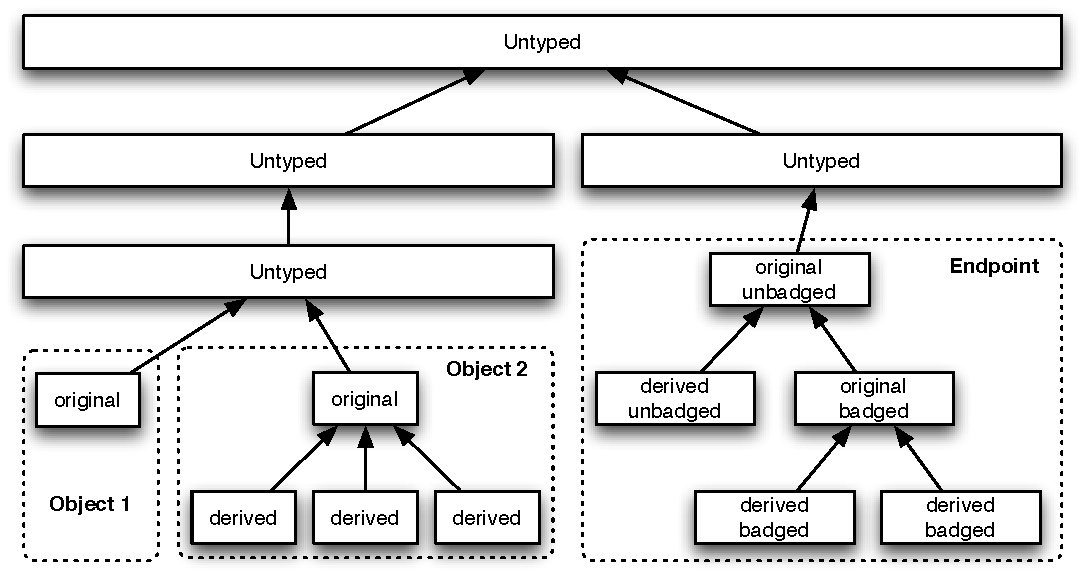
\includegraphics[width=0.8\textwidth]{figs/CDT}
  \end{center}
  \caption{Example capability derivation tree.}\label{fig:CDT}
\end{figure}

\autoref{fig:CDT} shows an example capability derivation tree that
illustrates a standard scenario: the top level is a large untyped
capability, the second level splits this capability into two regions
covered by their own untyped caps, both are children of the first
level.  The third level on the left is a copy of the level 2 untyped
capability.  Untyped capabilities when copied always create children,
never siblings.  In this scenario, the untyped capability was typed
into two separate objects, creating two capabilities on level 4, both
are the original capability to the respective object, both are
children of the untyped capability they were created from.

Ordinary original capabilities can have one level of derived
capabilities.  Further copies of these derived capabilities will
create siblings, in this case remaining on level 5. There is an
exception to this scheme for \obj{Endpoint} and \obj{Notification} capabilities --- they support an
additional layer of depth though \emph{badging}.
The original \obj{Endpoint} or \emph{Notification} capability will be unbadged. Using
the mint method, a copy of the capability with a specific \emph{badge} can be
created (see \autoref{s:ep-badge}, \autoref{s:notif-badge}). This new, badged capability to the same object is treated as
an original capability (the ``original badged endpoint capability'')
and supports one level of derived children like other capabilities.


\section{Deletion and Revocation}
\label{s:cspace-revoke}

Capabilities in seL4 can be deleted and revoked. Both methods
primarily affect capabilities, but they can have side effects on
objects in the system where the deletion or revocation results in the
destruction of the last capability to an object.

As described above, \apifunc{seL4\_CNode\_Delete}{cnode_delete} will
remove a capability from the specified CNode slot. Usually, this is
all that happens. If, however, it was the last typed capability to an
object, this object will now be destroyed by the kernel, cleaning up
all remaining in-kernel references and preparing the memory for
re-use.

If the object to be destroyed was a capability container, i.e.\ a TCB
or CNode, the destruction process will delete each capability held in
the container, prior to destroying the container. This may result in
the destruction of further objects if the contained capabilities are
the last capabilities.\footnote{The recursion is limited as if the last
capability to a CNode is found within the container, the found CNode
is not destroyed. Instead, the found CNode is made unreachable by
moving the capability pointing to the found CNode into the found cnode
itself, by swapping the capability with the first capability in the
found cnode, and then trying to delete the swapped capability
instead. This breaks the recursion.

The result of this approach is that deleting the last cap to the root
CNode of a CSpace does not recursively delete the entire
CSpace. Instead, it deletes the root CNode, and the branches of the
tree become unreachable, potentially including the deleting of some of
the unreachable CNode's caps to make space for the self-referring
capability. The practical consequence of this approach is that CSpace
deletion requires user-level to delete the tree leaf first if
unreachable CNodes are to be avoided. Alternatively, any resulting
unreachable CNodes can be cleaned up via revoking a covering untyped
capability, however this latter approach may be more complex to
arrange by construction at user-level.}

The \apifunc{seL4\_CNode\_Revoke}{cnode_revoke} method will
\apifunc{seL4\_CNode\_Delete}{cnode_delete} all CDT children of the
specified capability, but will leave the capability itself intact. If
any of the revoked child capabilities were the last capabilities to an
object, the appropriate destroy operation is triggered.

Note: \apifunc{seL4\_CNode\_Revoke}{cnode_revoke} may only partially
complete in two specific circumstances. The first being where a
CNode containing the last capability to the TCB of the thread
performing the revoke (or the last capability to the TCB itself) is
deleted as a result of the revoke. In this case the thread performing
the revoke is destroyed during the revoke and the revoke does not
complete. The second circumstance is where the storage containing the
capability that is the target of the revoke is deleted as a result of
the revoke. In this case, the authority to perform the revoke is
removed during the operation and the operation stops part way
through. Both these scenarios can be and should be avoided at
user-level by construction.

Note that for page tables and page directories
\apifunc{seL4\_CNode\_Revoke}{cnode_revoke} will not revoke frame
capabilities mapped into the address space.  They will only be
unmapped from the space.


\section{CSpace Addressing}
\label{s:cspace-addressing}

When performing a system call, a thread specifies to the kernel the
capability to be invoked by giving an address in its CSpace. This
address refers to the specific slot in the caller's CSpace that
contains the capability to be invoked.

CSpaces are designed to permit sparsity, and the process of looking-up
a capability address must be efficient. Therefore, CSpaces are
implemented as \emph{guarded page tables}.
% FIXME: need a references to justify the above decision

As explained earlier, a CSpace is a directed graph of \obj{CNode}
objects, and each \obj{CNode} is a table of slots, where each slot can
either be empty, or contain a capability, which may refer to another \obj{CNode}.
Recall from \autoref{s:sel4_internals} that the number of slots in a \obj{CNode}
must be a power of two. A \obj{CNode} is said to have a \emph{radix}, which is
the power to which two is raised in its size. That is, if a \obj{CNode} has
$2^k$ slots, its radix would be $k$.
The kernel stores a capability to the root \obj{CNode} of each thread's
CSpace in the thread's TCB. Conceptually, a \obj{CNode} capability
stores not only a reference to the \obj{CNode} to which it refers, but
also carries a \emph{guard} value, explained in
\autoref{sec:cap_address_lookup}.

\subsection{Capability Address Lookup}
\label{sec:cap_address_lookup}
Like a virtual memory address, a capability address is simply an
integer. Rather than referring to a location of physical memory (as
does a virtual memory address), a capability address refers to a
capability slot.  When looking up a capability address presented by a
userspace thread, the kernel first consults the \obj{CNode} capability
in the thread's TCB that defines the root of the thread's CSpace. It
then compares that \obj{CNode}'s \emph{guard} value against the most
significant bits of the capability address.  If the two values are
different, lookup fails. Otherwise, the kernel then uses the next
most-significant \emph{radix} bits of the capability address as an
index into the \obj{CNode} to which the \obj{CNode} capability
refers. The slot~$s$ identified by these next \emph{radix} bits might
contain another \obj{CNode} capability or contain something else
(including nothing).  If $s$ contains a \obj{CNode} capability~$c$ and
there are remaining bits (following the \emph{radix} bits) in the
capability address that have yet to be translated, the lookup process
repeats, starting from the \obj{CNode} capability~$c$ and using these
remaining bits of the capability address. Otherwise, the lookup
process terminates successfully; the capability address in question
refers to the capability slot~$s$.

\begin{figure}[tb]
    \begin{center}
        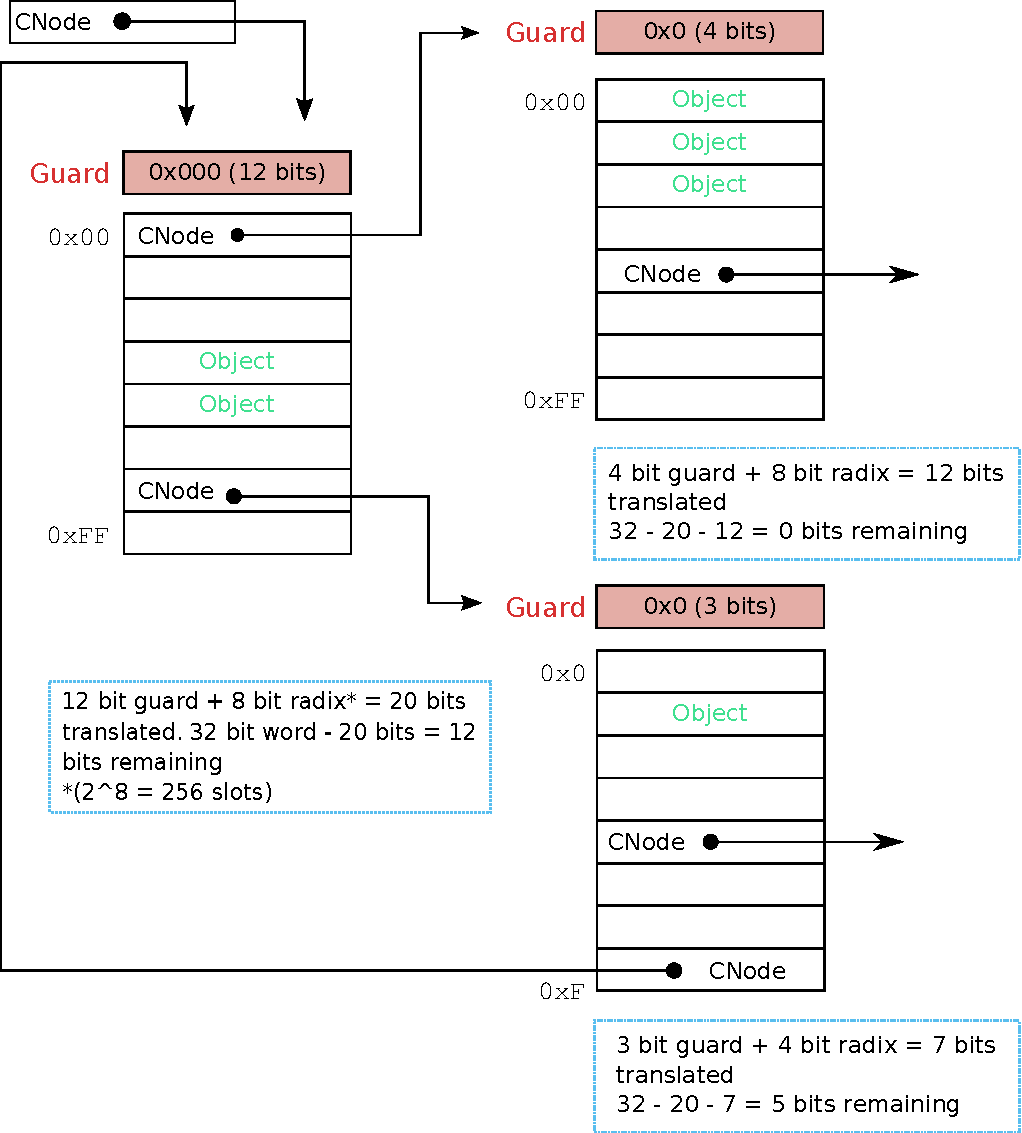
\includegraphics[scale=0.5]{figs/fig1-4.pdf}
        \caption{An example CSpace demonstrating object references at
          all levels, various guard and radix sizes and internal CNode
          references.}
        \label{fig1.4}
    \end{center}
\end{figure}

Figure \ref{fig1.4} demonstrates a valid CSpace with the following
features:
\begin{itemize}
\item a top level CNode object with a 12-bit guard set to 0x000 and
  256 slots;
\item a top level CNode with direct object references;
\item a top level CNode with two second-level CNode references;
\item second level CNodes with different guards and slot counts;
\item a second level CNode that contains a reference to a top level
  CNode;
\item a second level CNode that contains a reference to another CNode
  where there are some bits remaining to be translated;
\item a second level CNode that contains a reference to another CNode
  where there are no bits remaining to be translated; and
\item object references in the second level CNodes.
\end{itemize}

It should be noted that \autoref{fig1.4} demonstrates only what is
possible, not what is usually practical. Although the CSpace is legal,
it would be reasonably difficult to work with due to the small number
of slots and the circular references within it.


\subsection{Addressing Capabilities}
\label{sec:cap_addressing}

A capability address is stored in a CPointer (abbreviated CPTR), which
is an unsigned integer variable. Capabilities are addressed in
accordance with the translation algorithm described above.  Two
special cases involve addressing \obj{CNode} capabilities themselves
and addressing a range of capability slots.

Recall that the translation algorithm described above will traverse
\obj{CNode} capabilities while there are address bits remaining to be
translated. Therefore, in order to address a \obj{CNode} capability,
the user must supply not only a capability address but also specify
the maximum number of bits of the capability address that are to be
translated, called the \emph{depth limit}.

Certain methods, such as
\apifunc{seL4\_Untyped\_Retype}{untyped_retype}, require the user to
provide a range of capability slots. This is done by providing a base
capability address, which refers to the first slot in the range,
together with a window size parameter, specifying the number of slots
(with consecutive addresses, following the base slot) in the range.


\autoref{fig2.1} depicts an example CSpace. In order to illustrate
these ideas, we determine the address of each of the 10 capabilities
in this CSpace.

\begin{figure}[tb]
  \begin{center}
    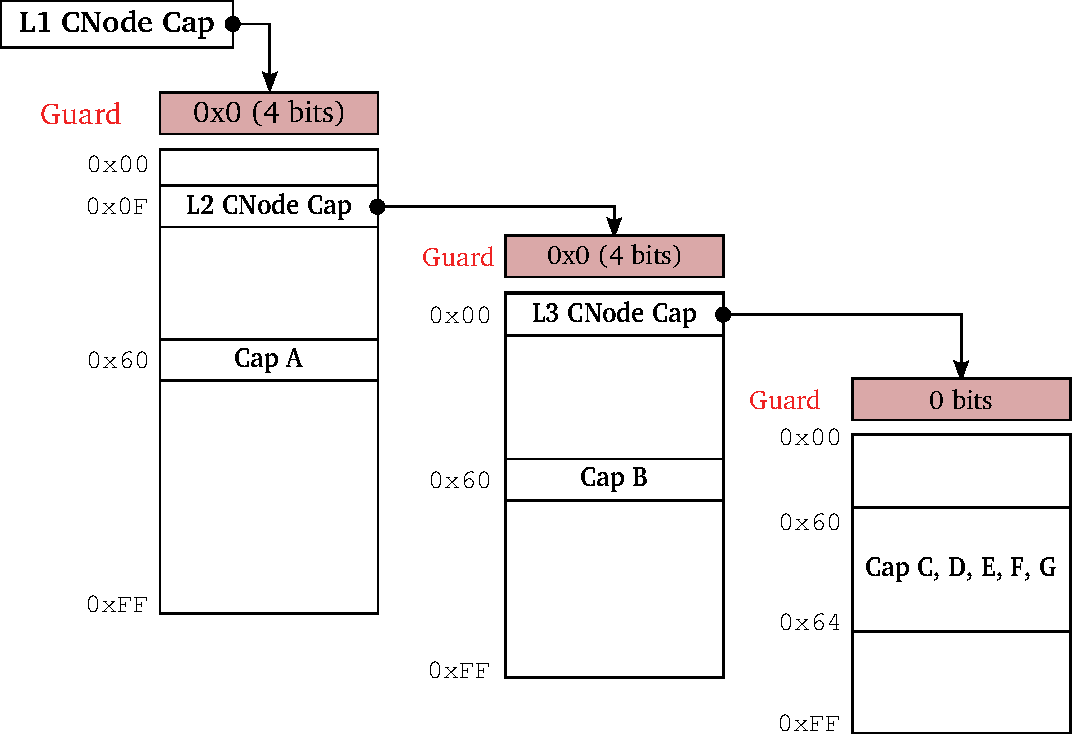
\includegraphics[scale=0.5]{figs/fig2-1.pdf}
    \caption{An arbitrary CSpace layout.}
    \label{fig2.1}
  \end{center}
\end{figure}


\begin{description}
\item[Cap A.] The first CNode has a 4-bit guard set to 0x0, and an
  8-bit radix. Cap A resides in slot 0x60 so it may be referred to by
  any address of the form 0x060xxxxx (where xxxxx is any number,
  because the translation process terminates after translating the
  first 12 bits of the address). For simplicity, we usually adopt the
  address 0x06000000.

\item[Cap B.] Again, the first CNode has a 4-bit guard set to 0x0, and
  an 8-bit radix. The second CNode is reached via the L2 CNode Cap.
  It also has a 4-bit guard of 0x0 and Cap B resides at index
  0x60. Hence, Cap B's address is 0x00F06000.  Translation of this
  address terminates after the first 24 bits.

\item[Cap C.] This capability is addressed via both CNodes. The third
  CNode is reached via the L3 CNode Cap, which resides at index 0x00
  of the second CNode. The third CNode has no guard and Cap C is at
  index 0x60.  Hence, its address is 0x00F00060. Translation of this
  address leaves 0 bits untranslated.

\item[Caps C--G.] This range of capability slots is addressed by
  providing a base address (which refers to the slot containing Cap C)
  of 0x00F00060 and a window size of 5.

\item[L2 CNode Cap.] Recall that to address a \obj{CNode} capability,
  the user must supply not only a capability address but also specify
  the depth limit, which is the maximum number of bits to be
  translated.  L2 CNode Cap resides at offset 0x0F of the first CNode,
  which has a 4-bit guard of 0x0.  Hence, its address is 0x00F00000,
  with a depth limit of 12 bits.

\item[L3 CNode Cap.] This capability resides at index 0x00 of the
  second CNode, which is reached by the L2 CNode Cap. The second CNode
  has a 4-bit guard of 0x0. Hence, the capability's address is
  0x00F00000 with a depth limit of 24 bits. Note that the addresses of
  the L2 and L3 CNode Caps are the same, but that their depth limits
  are different.
\end{description}

In summary, to refer to any capability (or slot) in a CSpace, the user
must supply its address. When the capability might be a CNode, the
user must also supply a depth limit.  To specify a range of capability
slots, the user supplies a starting address and a window size.

\section{Lookup Failure Description}
\label{sec:lookup_fail_desc}

When a capability lookup fails, a description of the failure is given
to either the calling thread or the thread's exception handler in its
IPC buffer.  The format of the description is always the same but may
occur at varying offsets in the IPC buffer depending on how the error
occurred.  The description format is explained below.  The first word
indicates the type of lookup failure and the meaning of later words
depend on this.

\subsection{Invalid Root}

A CSpace CPTR root (within which a capability was to be looked up)
is invalid. For example, the capability is not a \obj{CNode} cap.\\  \\

\begin{tabularx}{\textwidth}{XX}
  \toprule
  Data & Meaning \\
  \midrule
  \ipcbloc{Offset + 0} & \enummem{seL4\_InvalidRoot} \\
  \bottomrule
\end{tabularx}

\subsection{Missing Capability}

A capability required for an invocation is not present or does not
have sufficient rights. \\ \\

\begin{tabularx}{\textwidth}{XX}
  \toprule
  Data & Meaning \\
  \midrule
  \ipcbloc{Offset + 0} & \enummem{seL4\_MissingCapability} \\
    \ipcbloc{Offset + seL4\_CapFault\_BitsLeft} & Bits left \\
  \bottomrule
\end{tabularx}

\subsection{Depth Mismatch}

When resolving a capability, a CNode was traversed that resolved more
bits than was left to decode in the CPTR or a non-CNode capability was
encountered while there were still bits remaining to be looked up. \\ \\

\begin{tabularx}{\textwidth}{XX}
  \toprule
  Data & Meaning \\
  \midrule
  \ipcbloc{Offset + 0} & \enummem{seL4\_DepthMismatch} \\
  \ipcbloc{Offset + seL4\_CapFault\_BitsLeft} & Bits of CPTR remaining to decode \\
  \ipcbloc{Offset + seL4\_CapFault\_DepthMismatch\_BitsFound} & Bits that the current CNode being traversed resolved \\
  \bottomrule
\end{tabularx}

\subsection{Guard Mismatch}

When resolving a capability, a CNode was traversed with a guard size
larger than the number of bits remaining or the CNode's guard did not
match the next bits of the CPTR being resolved. \\ \\

\begin{tabularx}{\textwidth}{XX}
  \toprule
  Data & Meaning \\
  \midrule
  \ipcbloc{Offset + 0} & \enummem{seL4\_GuardMismatch} \\
    \ipcbloc{Offset + seL4\_CapFault\_BitsLeft} & Bits of CPTR remaining to decode \\
  \ipcbloc{Offset + seL4\_CapFault\_GuardMismatch\_GuardFound} & The CNode's guard \\
  \ipcbloc{Offset + seL4\_CapFault\_GuardMismatch\_BitsFound} & The CNode's guard size \\
  \bottomrule
\end{tabularx}


